\begin{multicols*}{2}
\begin{itemize}
\item The architecture selected for the problem definition was taken as SegNet(2015) because of it's simplicity 
\item Transfer training of the weights is performed and then fine tuned to attain the segmentation of the road. 
\end{itemize}
\begin{minipage}{0.25\textwidth}
\centering
  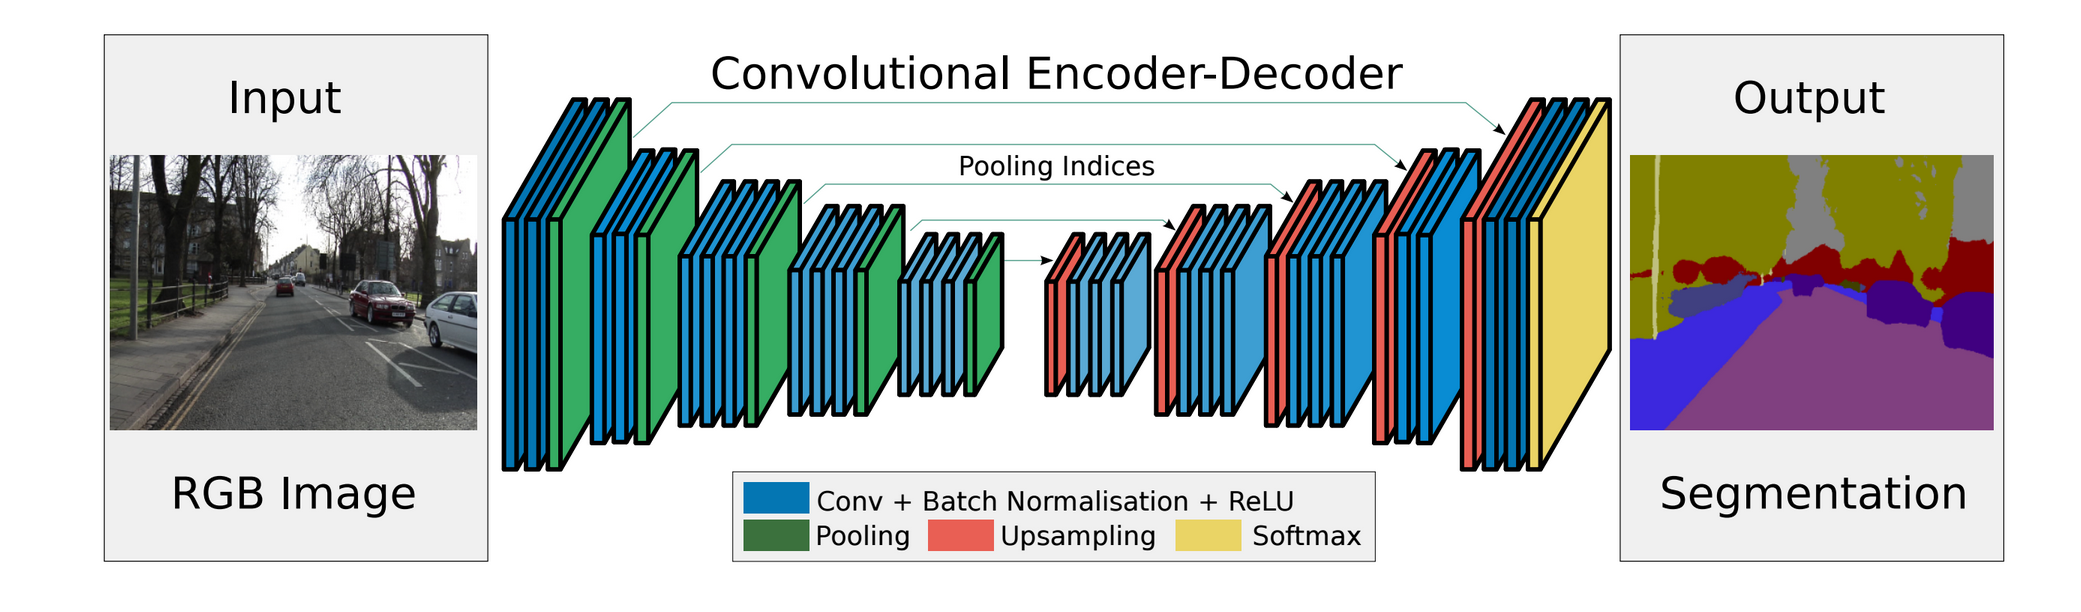
\includegraphics[width=0.75\linewidth]{images/scr2.png}
  \captionof{figure}{SegNet does not include any fully connected layer hence it is only convoluted. A sparse map of features is produced by the decoder which upsamples input produced by the encoder using encoders transferred pool indices. Then performs convolution with a trainable filter bank to densify the sparse feature map. Softmax classifier takes the final decoder output for pixel wise classification }
\end{minipage}
\end{multicols*}